\documentclass{beamer}

\usetheme{Stockton}
\usepackage{amssymb,graphicx,amsmath,graphicx,epstopdf,url,enumerate,wasysym}
 %\usepackage{beamerthemesplit} %// Activate for custom appearance

\title{Triangulation of the Cube}
\author{Ben Storlie}
\date{\today}

\begin{document}

\frame{\titlepage}

%\section[Outline]{}
%\frame{\tableofcontents}

\section{Introduction}
\frame
{
  \frametitle{Parameters}

  \begin{itemize}
  \item <1-> How many ways can an $n$-cube be divided into $n$-simplices?
  	\begin{itemize}
	\item <2-> where each simplex has the same volume,
	\item <3-> and no new vertices are made.\\
		\begin{itemize}
		\item <4-> (i.e. The vertices of each simplex are chosen from the 				vertices of the original cube.)
		\end{itemize}
	\end{itemize}
  \end{itemize}
}

\frame{
	\frametitle{What is a Simplex?}
	\bluebox{Simplex}{
	An {\bf$n$-simplex} is the simplest shape in $n$ dimensions.
	\begin{blackitemize}
	\item Includes points, line segments, triangles, and tetrahedra.
	\item In graph theory terms, an $n$-simplex is the complete graph on $n+1$ vertices.
\end{blackitemize}
	}
}



%These are images of simplices, showing how you just have to add a point and connect everybody.
\subsection{What is a Simplex?}

\frame{\frametitle{Zero Dimensions}
A Point
\centerline{\includegraphics[width=3in]{/Users/Ben/Documents/Thesis/Tetrahedra_in_Cubes/simple8.png}}}
\frame{\frametitle{Zero Dimensions}
add a new vertex...
\centerline{ \includegraphics[width=3in]{/Users/Ben/Documents/Thesis/Tetrahedra_in_Cubes/simple7.png}}}
\frame{\frametitle{One Dimension}
A Line Segment
\centerline{ \includegraphics[width=3in]{/Users/Ben/Documents/Thesis/Tetrahedra_in_Cubes/simple6.png}}}
\frame{\frametitle{One Dimension}
add a new vertex...
\centerline{ \includegraphics[width=3in]{/Users/Ben/Documents/Thesis/Tetrahedra_in_Cubes/simple5.png}}}
\frame{\frametitle{Two Dimensions}
A Triangle
\centerline{ \includegraphics[width=3in]{/Users/Ben/Documents/Thesis/Tetrahedra_in_Cubes/simple4.png}}}
\frame{\frametitle{Two Dimensions}
add a new vertex...
\centerline{ \includegraphics[width=3in]{/Users/Ben/Documents/Thesis/Tetrahedra_in_Cubes/simple3.png}}}
\frame{\frametitle{Three Dimensions}
A Tetrahedron
\centerline{ \includegraphics[width=3in]{/Users/Ben/Documents/Thesis/Tetrahedra_in_Cubes/simple2.png}}}
\frame{\frametitle{Three Dimensions}
A Tetrahedron
\centerline{ \includegraphics[width=3in]{/Users/Ben/Documents/Thesis/Tetrahedra_in_Cubes/simple1.png}}}
%%%%%%%%%%%%%%%%%


\subsection{How Do Simplices Fit into a Cube?}

\frame{\frametitle{How do Simplices Fit into a Cube?}}

\frame{\frametitle{Zero and One Dimensions}
\makebox[2em]{}A point in a point
\centerline{ 
\includegraphics[height=.25 in]{/Users/Ben/Documents/Thesis/Tetrahedra_in_Cubes/simplex1.png}}
\bigskip\bigskip\bigskip
\makebox[2em]{}A line segment in a line segment
\bigskip
\centerline{
\includegraphics[height=.25 in]{/Users/Ben/Documents/Thesis/Tetrahedra_in_Cubes/simplex2.png}}
}

\frame{\frametitle{Two Dimensions}
\centerline{\includegraphics[height=1.9 in]{/Users/Ben/Documents/Thesis/Tetrahedra_in_Cubes/square1.png}}}
\frame{\frametitle{Two Dimensions}
\centerline{\includegraphics[height=2 in]{/Users/Ben/Documents/Thesis/Tetrahedra_in_Cubes/square3.png}}}
\frame{\frametitle{Two Dimensions}
\centerline{\includegraphics[height=2 in]{/Users/Ben/Documents/Thesis/Tetrahedra_in_Cubes/square4.png}}}
\frame{\frametitle{Two Dimensions}
\centerline{\includegraphics[height=2 in]{/Users/Ben/Documents/Thesis/Tetrahedra_in_Cubes/square5.png}}}

\frame{\frametitle{Three Dimensions}
\centerline{\includegraphics[height=2 in]{/Users/Ben/Documents/Thesis/Tetrahedra_in_Cubes/cube1.png}}}
\frame{\frametitle{Three Dimensions}
\centerline{\includegraphics[height=2 in]{/Users/Ben/Documents/Thesis/Tetrahedra_in_Cubes/cube2.png}}}
\frame{\frametitle{Three Dimensions}
\centerline{\includegraphics[height=2 in]{/Users/Ben/Documents/Thesis/Tetrahedra_in_Cubes/cube3.png}}}
\frame{\frametitle{Three Dimensions}
\centerline{\includegraphics[height=2 in]{/Users/Ben/Documents/Thesis/Tetrahedra_in_Cubes/cube4.png}}}
\frame{\frametitle{Three Dimensions}
\centerline{\includegraphics[height=2 in]{/Users/Ben/Documents/Thesis/Tetrahedra_in_Cubes/cube5.png}}}

\frame{\frametitle{Three Dimensions}
\centerline{ A 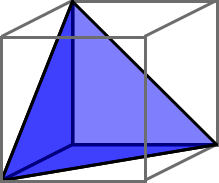
\includegraphics[height=1.2 in]{/Users/Ben/Documents/Thesis/Tetrahedra_in_Cubes/A.png}\quad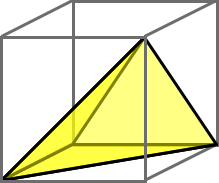
\includegraphics[height=1.2 in]{/Users/Ben/Documents/Thesis/Tetrahedra_in_Cubes/C.png} C}
\bigskip
\centerline{ BL \includegraphics[height=1.2 in]{/Users/Ben/Documents/Thesis/Tetrahedra_in_Cubes/cube3.png} \quad \includegraphics[height=1.2 in]{/Users/Ben/Documents/Thesis/Tetrahedra_in_Cubes/BR.png} BR}
}

\section{How to Fit These Tetrahedra in A Cube}

\frame{\frametitle{Pyramids}
\centerline{  \includegraphics[height=2 in]{/Users/Ben/Documents/Thesis/Tetrahedra_in_Cubes/pyramid1.png}\quad\includegraphics[height=2 in]{/Users/Ben/Documents/Thesis/Tetrahedra_in_Cubes/pyramid3.png} }
}

\end{document}
